\documentclass[border=1pt,tikz,varwidth=\maxdimen]{standalone}

\usetikzlibrary{positioning,calc,trees,arrows}

\usepackage{amsmath,mathtools}

\begin{document}
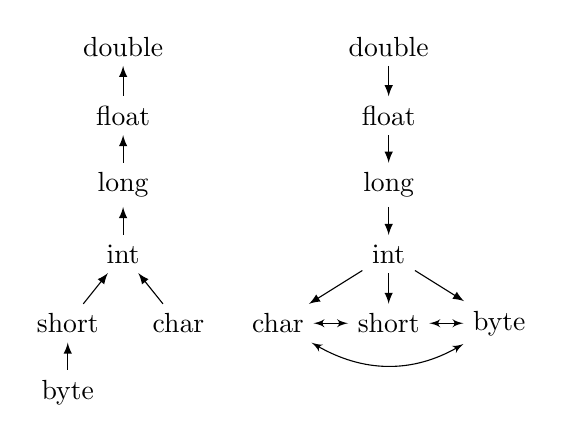
\begin{tikzpicture}[
  level distance = 2.5em,
  sibling distance = 4em,
  positive-arrow/.style={edge from parent/.style={latex-,solid,draw}},
  negative-arrow/.style={edge from parent/.style={-latex,solid,draw}},
  ]
  \node (widening) {double}
  child[positive-arrow] {
    node {float}
    child {
      node {long}
      child {
        node {int}
        child {
          node {short}
          child {
            node {byte}
          }
        }
        child {
          node {char}
        }
      }
    }
  };

  \node[right=6em of widening] (narrowing) {double}
  child[negative-arrow] {
    node {float}
    child {
      node {long}
      child {
        node {int}
        child {
          node (narrowing-char) {char}
        }
        child {
          node (narrowing-short) {short}
        }
        child {
          node (narrowing-byte) {byte}
        }
      }
    }
  };

  \draw [latex'-latex'] (narrowing-char) -- (narrowing-short);
  \draw [latex'-latex'] (narrowing-short) -- (narrowing-byte);
  \draw [latex'-latex'] (narrowing-char) edge[out=330,in=210] (narrowing-byte);
\end{tikzpicture}
\end{document}
